\documentclass[tikz,border=3pt]{standalone}
\usepackage[T1]{fontenc}
\usepackage{newtxtext,newtxmath}
\usetikzlibrary{arrows.meta,calc}
\definecolor{ink}{HTML}{23343F}
\definecolor{blue}{HTML}{2276A0}
\definecolor{teal}{HTML}{087F78}
\definecolor{orange}{HTML}{C46B2C}
\definecolor{muted}{HTML}{4C5D67}
\definecolor{rule}{HTML}{D6DFE3}
\begin{document}
\begin{tikzpicture}[font=\fontsize{8}{9.6}\selectfont,text=ink,line cap=round,
 >={Stealth[length=1.5mm,width=1.05mm]},
 head/.style={font=\bfseries\fontsize{8.8}{10}\selectfont,anchor=west},
 note/.style={font=\fontsize{7.2}{8.6}\selectfont,text=muted},
 tiny/.style={font=\fontsize{6.8}{8}\selectfont,text=muted},
 flow/.style={->,draw=muted,line width=.65pt},
 card/.style={draw=rule,line width=.5pt,rounded corners=1.5pt,fill=white},
 bus/.style={draw=ink,line width=1.3pt},
 pmu/.style={draw=blue,fill=blue!8,line width=.7pt}]
\path[use as bounding box] (0,0) rectangle (17.7,10.6);

% (a) Problem and observed input. One clock, two interventions, a persistent response.
\fill[teal!4,rounded corners=1.5pt] (.05,8.4) rectangle (8.5,10.55);
\node[head] at (.25,10.3) {(a) A new intervention before recovery ends};
\node[note,anchor=west] at (.3,9.56) {A};
\node[note,anchor=west] at (.3,9.13) {B};
\draw[rule] (1.0,9.56)--(7.97,9.56) (1.0,9.13)--(7.97,9.13);
\fill[teal] (1.65,9.45) rectangle (3.6,9.67);
\fill[orange] (5.55,9.02) rectangle (7.25,9.24);
\node[tiny,above] at (1.65,9.69) {ON};
\node[tiny,above] at (3.6,9.69) {OFF};
\node[tiny,anchor=east,fill=teal!4,inner sep=1pt] at (5.35,9.13) {new ON};
\draw[teal,densely dashed,line width=.85pt] (3.6,9.56)
 .. controls (4.0,10.0) and (4.2,9.15) .. (4.65,9.56)
 .. controls (5.0,9.8) and (5.15,9.33) .. (5.55,9.56)
 .. controls (5.95,9.71) and (6.2,9.45) .. (6.55,9.56)--(7.97,9.56);
\node[note,anchor=west] at (.3,8.65) {Restored input $\ne$ equilibrium state};
\node[note,anchor=east,text=teal] at (8.15,8.65) {recovery persists};

\node[head] at (9.05,10.3) {Observed PMU stream};
% Phasor instrument icon.
\draw[rule] (9.65,9.19) circle (.37);
\draw[rule] (9.17,9.19)--(10.13,9.19) (9.65,8.73)--(9.65,9.66);
\draw[blue,->,line width=.85pt] (9.65,9.19)--(9.87,9.5);
\draw[orange,->,line width=.85pt] (9.65,9.19)--(9.98,9.03);
\node[anchor=west] at (10.4,9.55) {8 PMUs \quad $r_k\in\mathbb R^{47}$ \quad 30 reports/s};
\node[note,anchor=west] at (10.4,9.13) {$|V|,\angle V$ \quad $|I|,\angle I$ \quad $f,\dot f$};
\node[note,anchor=west] at (10.4,8.7) {Mapped terminals; causal instrument memory};
% Separate routes for one-time context fitting and the new scored report.
\draw[flow] (10.55,8.4)--(10.55,8.13)--(2.75,8.13)--(2.75,7.73);
\node[tiny,fill=white,inner sep=1.5pt] at (6.55,8.13) {startup prefix: operating context and noise};
\draw[flow,blue] (14.95,8.4)--(14.95,7.73);
\node[tiny,anchor=west,text=blue] at (15.1,8.05) {each report};

% (b) Implemented pipeline: three aligned cards, external arrows only.
\foreach \xa/\xb/\cc in {.05/5.48/blue,6.13/11.56/teal,12.21/17.64/orange}{
 \path[card] (\xa,2.98) rectangle (\xb,7.72);
 \fill[\cc!7] (\xa,7.02) rectangle (\xb,7.72);
 \draw[\cc,line width=1.1pt] (\xa,7.72)--(\xb,7.72);
}
\node[head] at (.25,7.42) {(b) 1\quad Network physics};
\node[head] at (6.33,7.42) {2\quad Competing event histories};
\node[head] at (12.41,7.42) {3\quad Conditional Bayesian evidence};
\node[note,anchor=west] at (.27,6.78) {Graph, machines, load law and instruments};
\node[note,anchor=west] at (6.35,6.78) {9 load buses + 9 lines; unknown onset};
\node[note,anchor=west] at (12.43,6.78) {Score the same report under each history};

% Generic electrical motif: buses, generator, load, line breaker, mapped PMU.
\draw[bus] (.85,5.78)--(.85,6.33) (2.1,5.78)--(2.1,6.33)
 (3.45,5.78)--(3.45,6.33) (4.65,5.78)--(4.65,6.33);
\draw[ink,line width=.65pt] (.85,6.05)--(2.1,6.05)--(2.64,6.05)
 (3.02,6.05)--(4.65,6.05) (.85,6.05)--(.85,6.52)--(4.65,6.52)--(4.65,6.05);
\draw[orange,line width=.95pt] (2.64,6.05)--(2.99,6.29);
\draw[orange,fill=white] (2.64,6.05) circle (.035) (3.02,6.05) circle (.035);
\draw[blue] (.4,6.05) circle (.18);
\draw[ink] (.58,6.05)--(.85,6.05);
\draw[blue,line width=.55pt] (.27,6.05) .. controls (.32,6.23) and (.38,5.87) .. (.45,6.05) .. controls (.48,6.14) and (.5,6.05) .. (.53,6.05);
\draw[orange,->,line width=.85pt] (2.1,6.05)--(2.1,5.46);
\node[tiny,text=orange,below] at (2.1,5.43) {$\Delta P,\Delta Q$};
\node[pmu,rectangle,inner sep=2pt,font=\fontsize{6.5}{7}\selectfont] at (4.65,5.57) {PMU};
\draw[blue] (4.65,5.79)--(4.65,5.95);
\node[tiny] at (3.4,5.57) {$q$: line mode};
\node[align=center] at (2.76,4.91) {$\dot x=f_q(x,z,u),\qquad 0=g_q(x,z,u)$};
\node at (2.76,4.43) {$I_{\rm bus}=Y_qV,\quad I_{\rm term}=Y_{{\rm term},q}V$};
\draw[rule] (.36,4.1)--(5.17,4.1);
\node[note] at (2.76,3.81) {Local DAE reduction + report formation};
\node at (2.76,3.42) {$T_o,J_o,g_o,u_o,j_o,v_o$};
\draw[flow] (5.53,5.45)--(6.08,5.45);

% Hypothesis stack: waveform icons are schematic, not measured traces.
\foreach \yy/\txt/\cc in {6.13/{No new intervention}/muted,5.6/{Recovery of A}/teal,5.07/{Recovery + new B}/orange}{
 \fill[\cc!5,rounded corners=1pt] (6.4,{\yy-.2}) rectangle (11.28,{\yy+.2});
 \fill[\cc] (6.62,\yy) circle (.047);
 \node[note,text=\cc,anchor=west] at (6.82,\yy) {\txt};
}
\draw[muted,line width=.7pt] (9.9,6.13)--(11.02,6.13);
\draw[teal,dashed,line width=.8pt] (9.9,5.6) .. controls (10.13,6.0) and (10.3,5.26) .. (10.54,5.6) .. controls (10.7,5.77) and (10.85,5.5) .. (11.02,5.6);
\draw[orange,line width=.8pt] (9.9,5.07)--(10.16,5.07)--(10.16,5.24) .. controls (10.45,5.42) and (10.6,4.84) .. (11.02,5.07);
\node at (8.85,4.48) {$(m_h,d_h,\mu_h,v_h,\pi_h)$};
\node[note] at (8.85,4.08) {State--severity dependence is retained};
\draw[rule] (6.43,3.83)--(11.26,3.83);
\node[text=teal] at (8.85,3.53) {$x(\kappa^+)=x(\kappa^-)$};
\node[note] at (8.85,3.19) {Restore the operator; carry the state};
\draw[flow] (11.61,5.45)--(12.16,5.45);

% Scoring, marginalization, model weighting and causality contract.
\node at (14.93,6.17) {$e_h=r_k-J_om_h-j_o,\quad s_h=J_od_h+v_o$};
\node at (14.93,5.57) {$L_{h,k}=\displaystyle\int_l^u\!\mathcal N(e_h;s_ha,S_o)\,p_h(a)\,da$};
\node[note] at (14.93,5.08) {Integrate load severity; lines use switched models};
\draw[rule] (12.51,4.78)--(17.34,4.78);
\node at (14.93,4.46) {$\pi_{h,k}\propto L_{h,k}\,\pi_{h,k}^{\rm prior}$};
\node[note] at (14.93,4.05) {Normalize within each network hypothesis};
\node[note] at (14.93,3.68) {Outer weights: finite R/X alternatives};
\node[tiny] at (14.93,3.27) {Replay replaces suffix evidence; pruning is approximate};
% Posterior feedback and a distinct output route; no crossing of card content.
\draw[->,teal,line width=.65pt] (14.0,2.98)--(14.0,2.62)--(8.85,2.62)--(8.85,2.98);
\node[tiny,text=teal,fill=white,inner sep=1.3pt] at (11.4,2.62) {updated histories $\rightarrow$ next report};
\draw[flow] (16.85,2.98)--(16.85,2.3);
\draw[->,blue,dashed,line width=.6pt] (2.75,2.98)--(2.75,2.3);
\node[tiny,anchor=west,text=blue] at (2.95,2.65) {nominal source signatures};

% (c) A parallel explanatory diagnostic and the actual publication output.
\path[card,fill=blue!2] (.05,.4) rectangle (8.55,2.3);
\path[card,fill=orange!2] (9.1,.4) rectangle (17.64,2.3);
\node[head] at (.25,2.02) {(c) Explain source ambiguity};
\node[note,anchor=east] at (8.31,2.02) {Nominal diagnostic};
% Two close directions illustrate competing signatures in observation space.
\draw[rule] (.55,.93)--(2.05,.93) (.55,.93)--(.55,1.66);
\draw[blue,->,line width=.85pt] (.55,.93)--(1.82,1.54);
\draw[orange,->,line width=.85pt] (.55,.93)--(1.92,1.28);
\node at (5.13,1.45) {$\widetilde Q_{i\mid j}=\min_b\,\tfrac12\|\mu_i-\mu_j(b)\|_{\Sigma^{-1}}^2$};
\node[note] at (4.29,.77) {V versus V+I; correlated reports; not a publication gate};
\node[head] at (9.3,2.02) {4\quad Publish on the current report clock};
\node at (11.22,1.52) {$M_c$: active};
\node at (14.7,1.52) {$\Gamma_c$: originating cause};
\node[note] at (13.38,1.09) {Calibrated thresholds + consecutive-report confirmation};
\node[text=orange,font=\bfseries\fontsize{7.7}{9}\selectfont] at (13.38,.66)
 {Event type \quad Source \quad Onset estimate \quad Restoration};
\node[tiny,anchor=west] at (.1,.13) {Generic electrical motif and schematic traces. Finite histories and shared covariance approximations produce approximate attribution weights.};
\end{tikzpicture}
\end{document}
